\section{ 基于Arduino的定时器库函数}
\subsection{基于Arduino的Timer定时器概述}

ESP32 提供 2 个硬件定时器组，每组有 2 个硬件通用定时器，即 ESP32 芯片内置 4 个硬件通用定时器，分别对应序号：0、1、2、3。

每个定时器包含 1 个 16 位预分频器和 1 个 64 位可自动重载向上/向下计数器。

ESP32 的计数基频为 80\,MHz，预分频系数为 80 可得到 1\,MHz 的计数信号，每个计数信号的周期为 1\,$\mu$s，即每个计数单位为 1\,$\mu$s。

\subsection{定时器的初始化流程}

初始化一个定时器对象：\texttt{timerBegin()}，返回 \texttt{hw\_timer\_t} 类型的定时器对象。

设置定时器中断：\texttt{timerAttachInterrupt()}。

配置定时器参数：\texttt{timerAlarmWrite()}。

使能开启定时器：\texttt{timerAlarmEnable()}。

\subsection{定时器中断回调各函数具体介绍}
\subsubsection{ 定时器初始化函数 }
\begin{figure}[h]
    \centering
    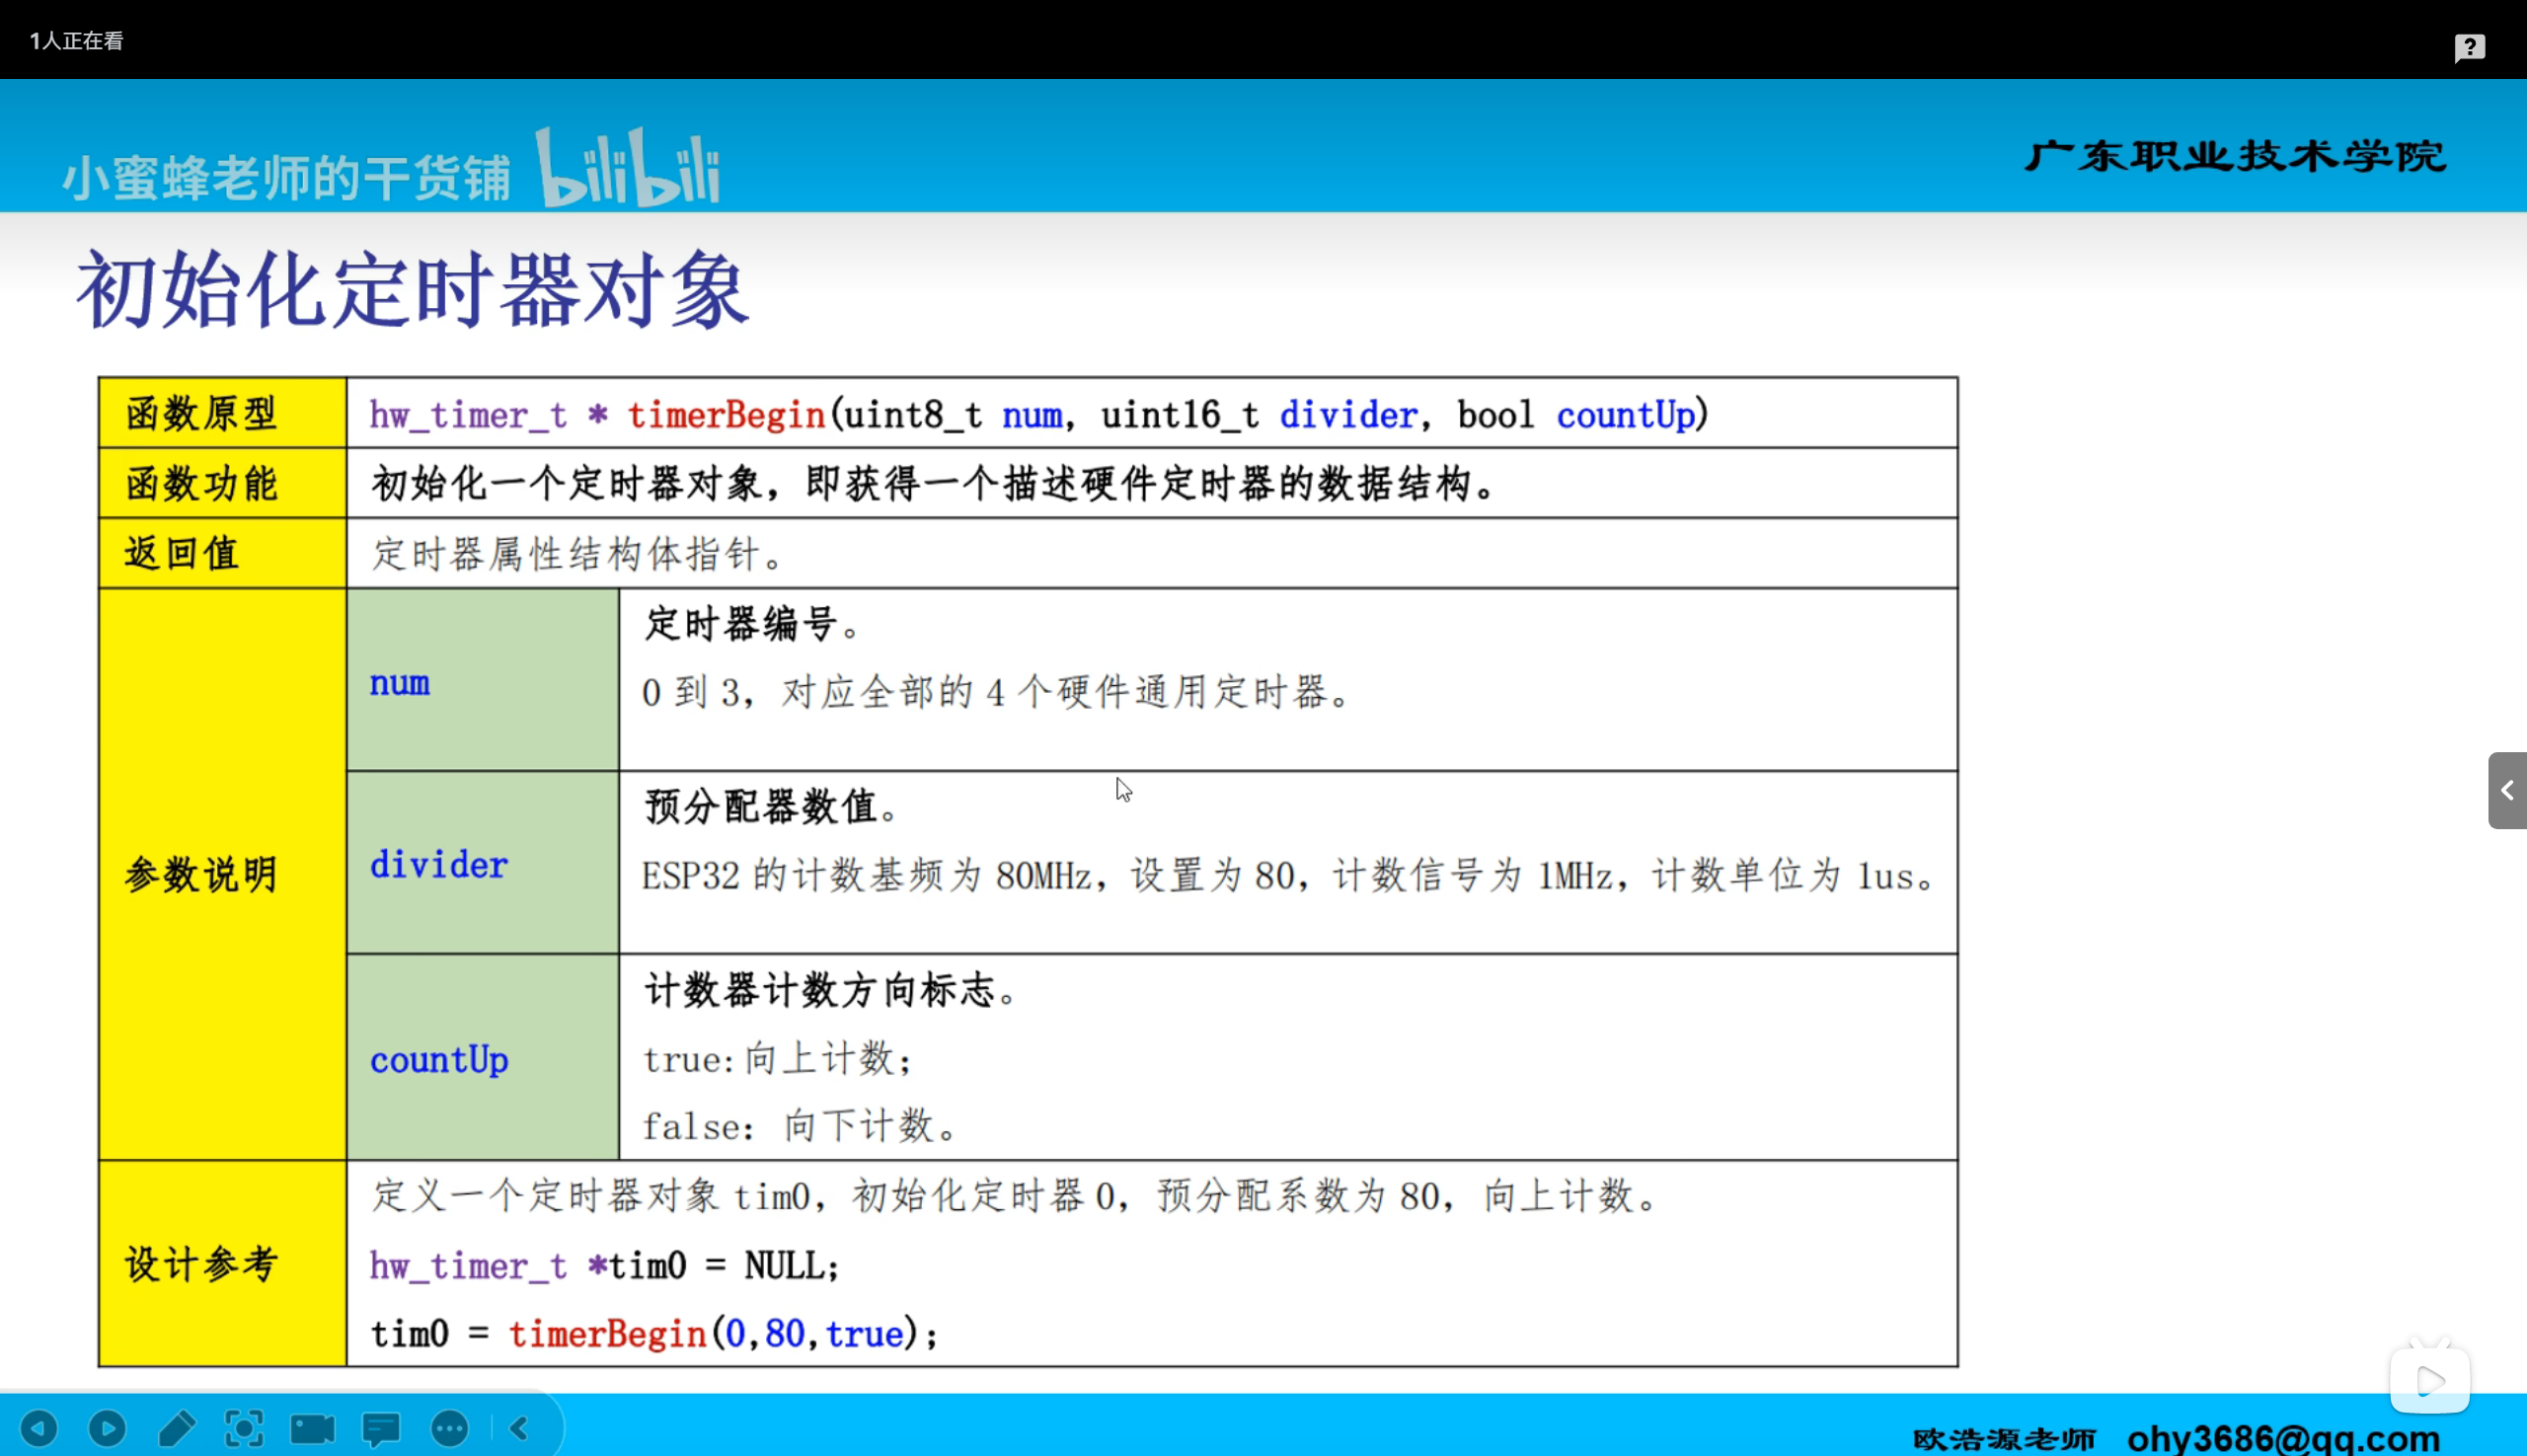
\includegraphics[width=0.6\textwidth]{Figures/TimerInit.png}
    \caption{timerBegin}
\end{figure}
函数名为: \textit{\textbf{timerBegin(参数一,参数二,参数三)} }.
\begin{itemize}
    \item 参数一:要对哪一个定时器进行操作(有定时器0,定时器一、二、三等等)
    \item 参数二:要设置的预分配系数
    \item 参数三:设置计数器计数计数方向,规定向上计数还是向下计数
    \item 返回值:返回值是一个存储着刚才配置信息的结构体指针
\end{itemize}
\newpage
\subsection{ 定时器参数配置 }
\begin{figure}[h]
    \centering
    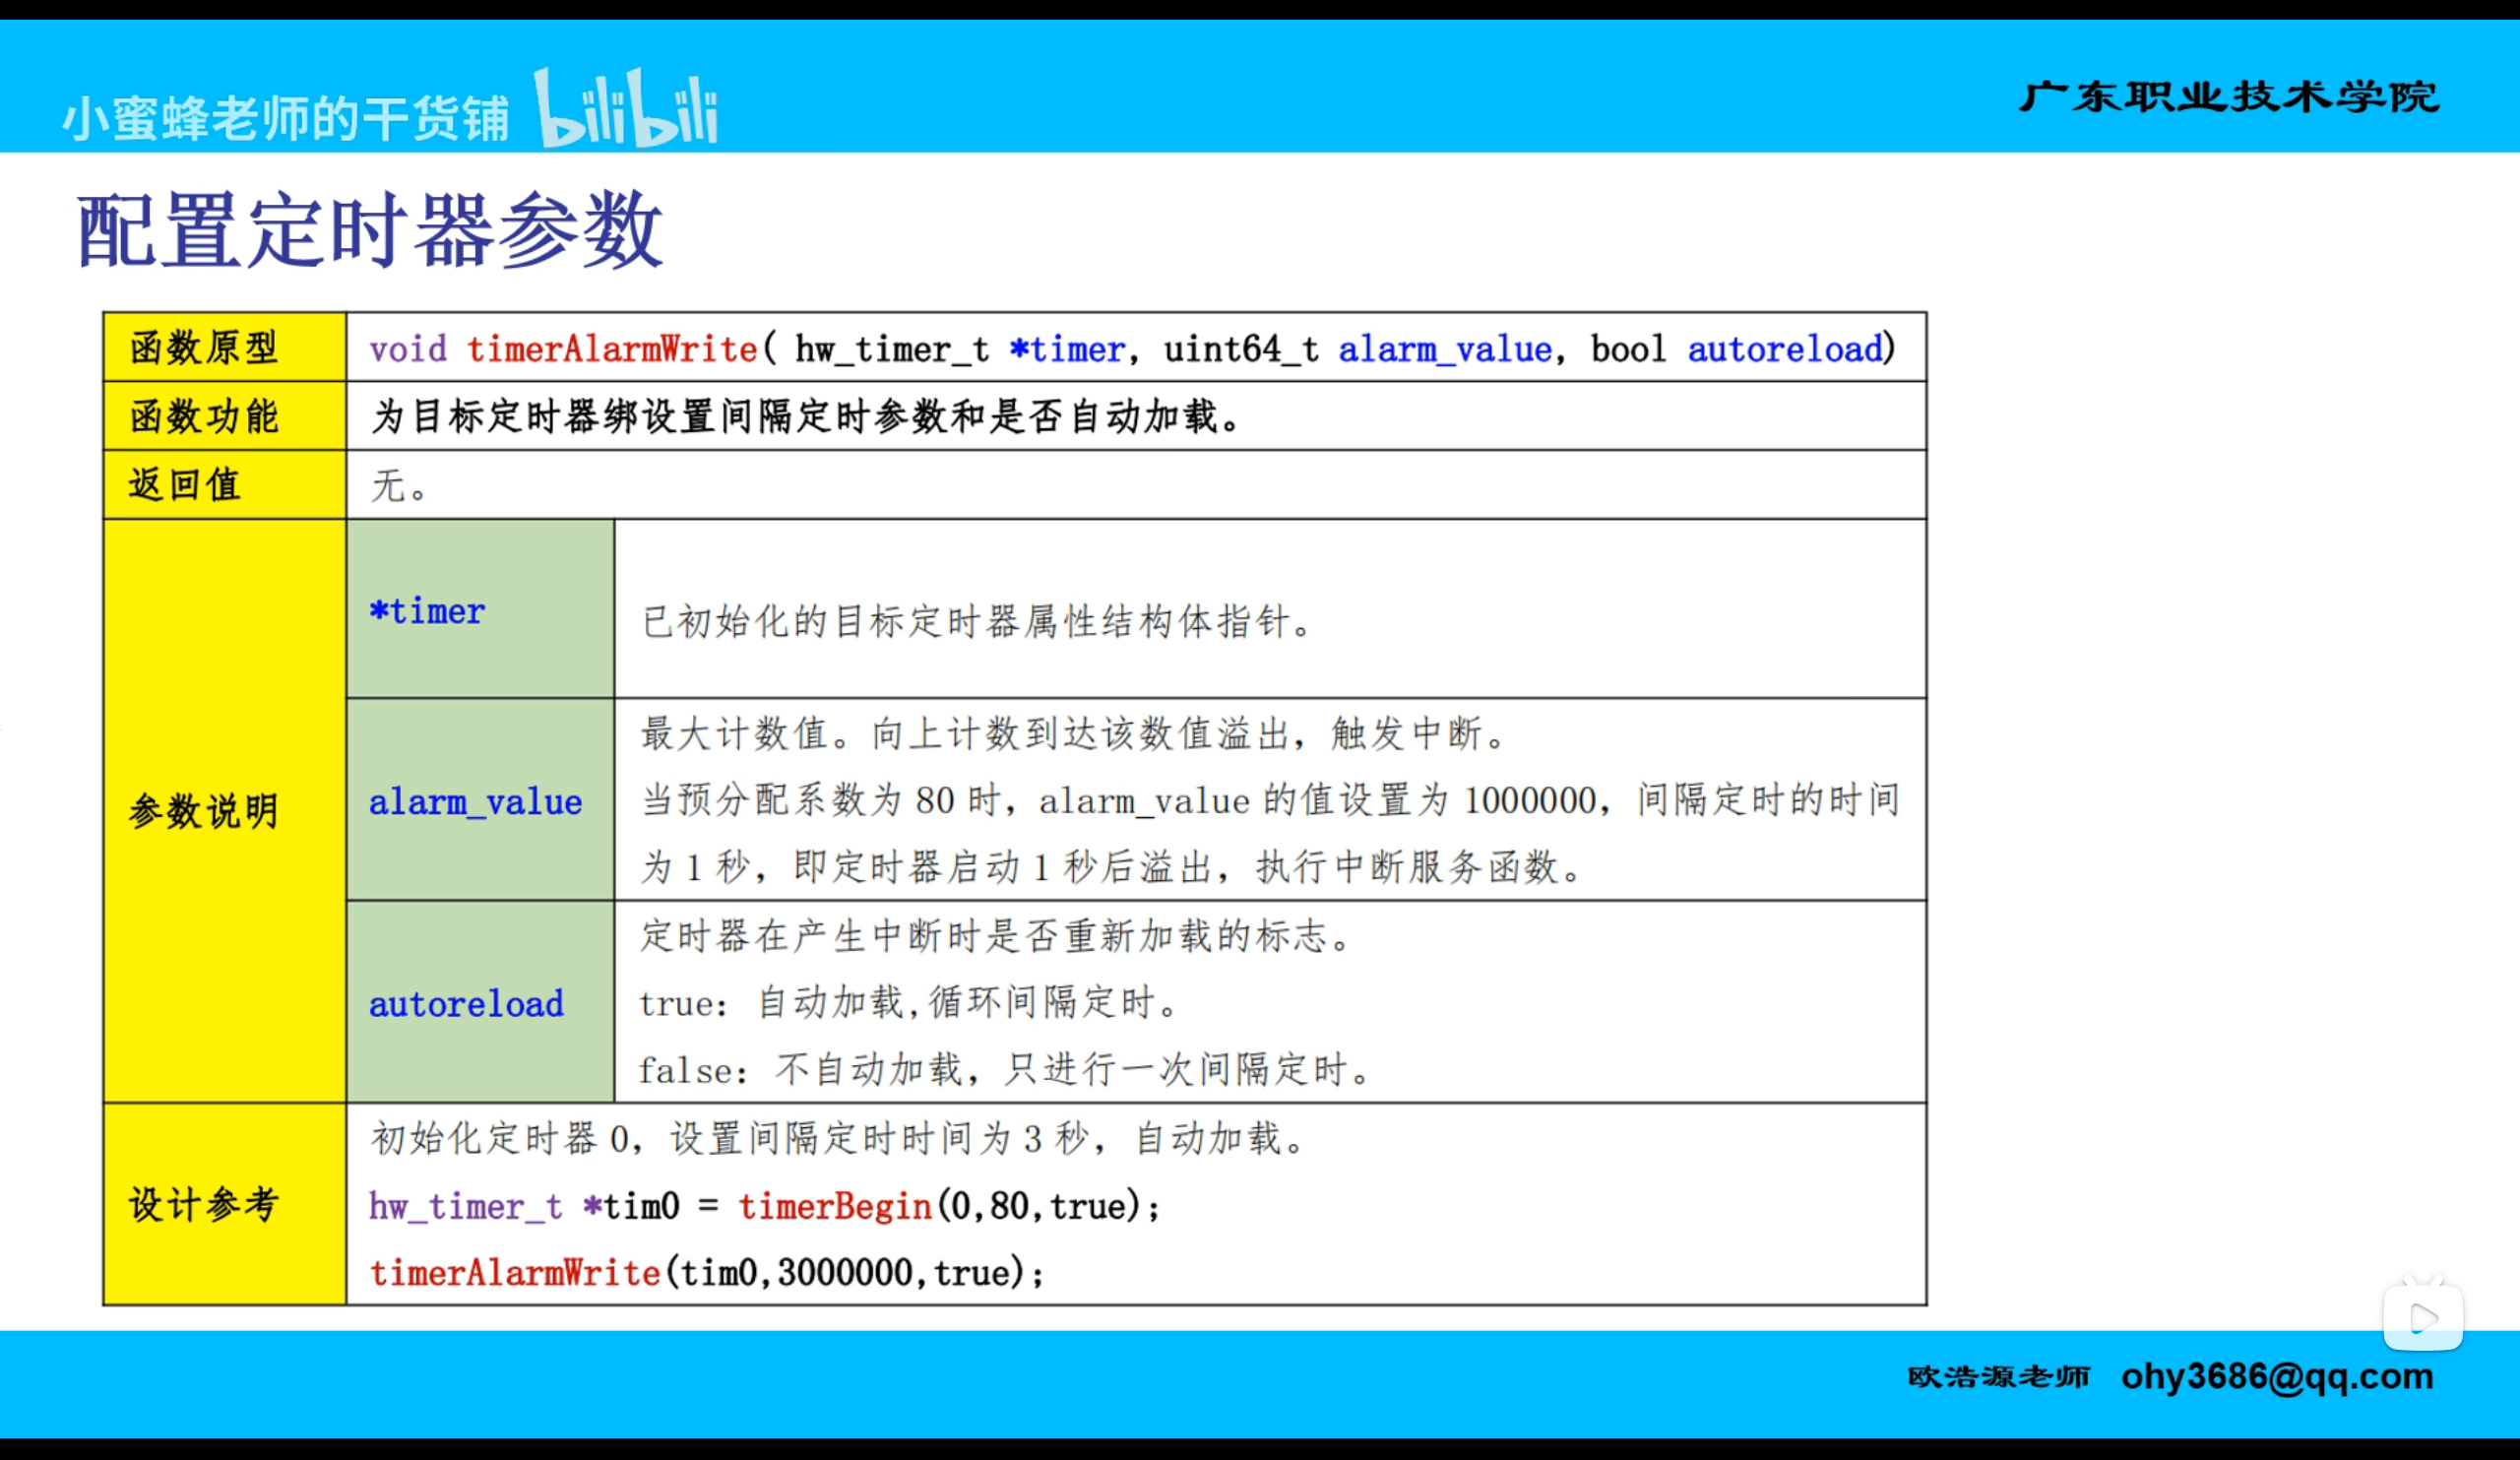
\includegraphics[width=\textwidth]{Figures/Timer_Perimiter.png}
    \caption{配置定时器参数}    
\end{figure}
函数名为: \textit{\textbf{timerAlarmWrite(参数一,参数二,参数三)}}.
\begin{itemize}
    \item 参数一:填写着要配置中断的时钟的信息的结构体指针(例如样例中给的*tim0)
    \item 参数二:最大计数值
    \item 参数三:决定是否循环调用计时器中断函数
\end{itemize}
\newpage
\subsubsection{ 定时器中断配置函数 }
\begin{figure}[h]
    \centering
    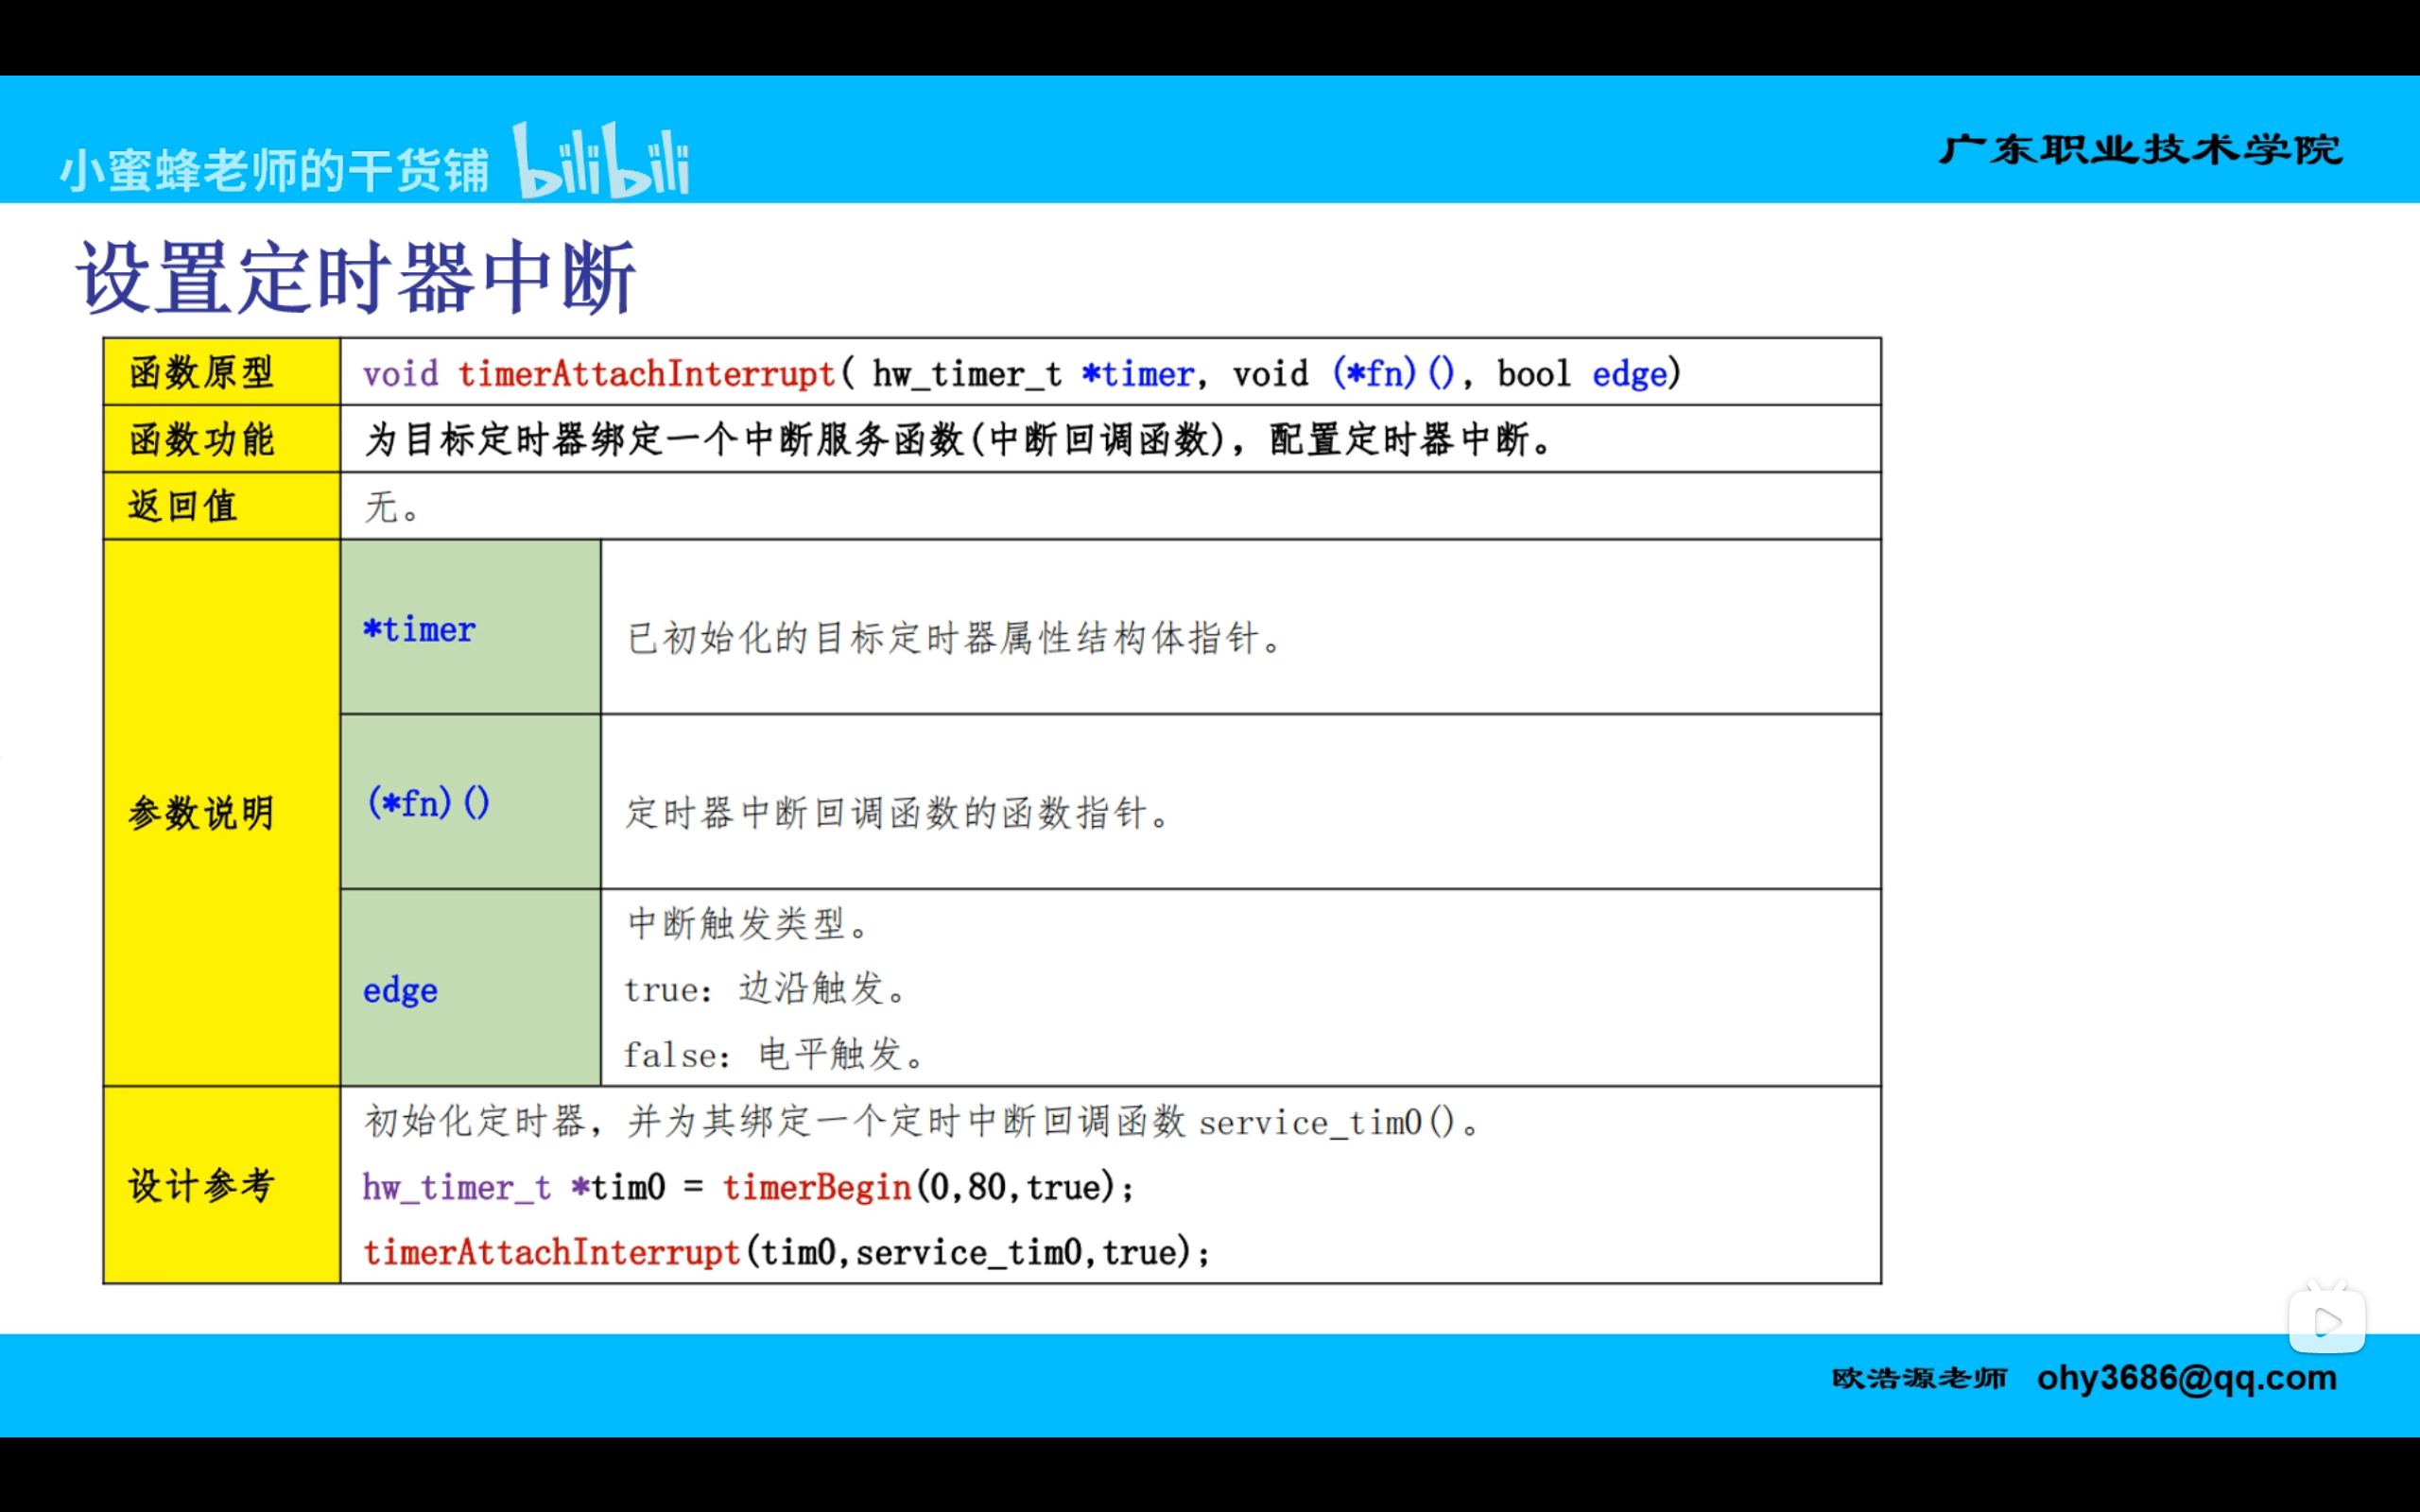
\includegraphics[width=\textwidth]{Figures/Timer_Interrupt.png}
    \caption{定时器中断配置函数}    
\end{figure}
函数名为: \textit{\textbf{void timerAttachInterrupt(参数一,参数二,参数三)}}.
\begin{itemize}
    \item 参数一:填写着要配置中断的时钟的信息的结构体指针(例如样例中给的*tim0)
    \item 参数二:发生中断时要调用的函数指针
    \item 参数三:触发中断的方式(边沿触发和电平触发)
\end{itemize}


